\documentclass[10pt,aspectratio=169]{beamer}

% Tema moderno y elegante Metropolis
\usetheme{metropolis}
\metroset{progressbar=frametitle, block=fill}

% Paquetes esenciales
\usepackage[spanish,es-nodecimaldot]{babel}
\usepackage[utf8]{inputenc}
\usepackage{amsmath,amssymb,amsfonts}
\usepackage{graphicx}
\usepackage{booktabs}
\usepackage{microtype}
\usepackage{tikz}
\usetikzlibrary{positioning}

% Directorio de figuras
\graphicspath{{graficas/}}

% Paleta de colores personalizada de alto contraste
\definecolor{NavyDark}{HTML}{0B2545}
\definecolor{NavyMedium}{HTML}{134074}
\definecolor{TealAccent}{HTML}{2A9D8F}
\definecolor{CoralAccent}{HTML}{E63946}
\definecolor{SandLight}{HTML}{F8F9FA}
\definecolor{GrayDark}{HTML}{2B2D42}
\definecolor{PurpleAccent}{HTML}{7A5195}

\setbeamercolor{palette primary}{bg=NavyDark,fg=white}
\setbeamercolor{palette secondary}{bg=NavyMedium,fg=white}
\setbeamercolor{progress bar}{fg=TealAccent,bg=NavyMedium!30}
\setbeamercolor{title separator}{fg=TealAccent}
\setbeamercolor{block title}{bg=NavyMedium,fg=white}
\setbeamercolor{block body}{bg=SandLight,fg=GrayDark}
\setbeamercolor{alerted text}{fg=CoralAccent}

% Título y Metadatos
\title{Diagnóstico del Aprendizaje y Parada Temprana}
\subtitle{Prevención de Sobreajuste, Checkpointing Óptimo y Evaluación de Predicciones}
\author{\textbf{Laboratorio de Inteligencia Artificial} --- PyTorch Demanda}
\date{\today}
\institute{Deep Learning \& Modelado Predictivo (\texttt{red\_neuronal.py})}

\begin{document}

% -----------------------------------------------------------------------------
% SLIDE 1: PORTADA
% -----------------------------------------------------------------------------
\begin{frame}
  \titlepage
\end{frame}

% -----------------------------------------------------------------------------
% SLIDE 2: MOTIVACIÓN Y EL DILEMA DEL NÚMERO DE ÉPOCAS
% -----------------------------------------------------------------------------
\begin{frame}{El Problema: ¿Por qué Entrenar a Ciegas es Peligroso?}
  \begin{columns}[T]
    \begin{column}{0.48\textwidth}
      \begin{block}{El Enfoque Tradicional Fijo}
        \scriptsize
        Fijar un número arbitrario de épocas (ej. \texttt{EPOCAS = 100}) plantea un dilema irresoluble a priori:
        \begin{itemize}
          \item \textbf{Muy pocas épocas}: El modelo se queda en \textbf{subajuste} (\textit{underfitting}), sin extraer patrones no lineales.
          \item \textbf{Demasiadas épocas}: La red memoriza el ruido muestral en \textbf{sobreajuste} (\textit{overfitting}).
        \end{itemize}
      \end{block}

      \vspace{-0.1cm}
      \begin{block}{La Solución Natural}
        \scriptsize
        Transformar el criterio de parada en un \textbf{mecanismo dinámico}:
        \[
          t_{\text{stop}} = \min \left\{ t \;\middle|\; \Delta t_{\text{sin mejora}} \ge P \right\}
        \]
        donde $P$ es la \textbf{paciencia} del optimizador.
      \end{block}
    \end{column}

    \begin{column}{0.48\textwidth}
      \begin{alertblock}{Riesgos de Usar el Último Modelo}
        \scriptsize
        \begin{itemize}
          \item En la época final $E=100$, los pesos $\theta_{100}$ rara vez son los mejores.
          \item En problemas reales, la pérdida de validación oscila y con frecuencia \textbf{empeora al final}.
          \item \textbf{Conclusión clave}: Necesitamos guardar el mejor punto histórico $\theta^*$ (\textit{checkpointing}) y cortar el cómputo cuando ya no hay ganancia real.
        \end{itemize}
      \end{alertblock}
    \end{column}
  \end{columns}
\end{frame}

% -----------------------------------------------------------------------------
% SLIDE 3: FUNDAMENTO MATEMÁTICO DE EARLY STOPPING
% -----------------------------------------------------------------------------
\begin{frame}{Fundamento Teórico: Regularización Implícita}
  \begin{columns}[T]
    \begin{column}{0.50\textwidth}
      \begin{block}{Equivalencia con Regularización $L_2$ (Weight Decay)}
        \scriptsize
        Existe una equivalencia matemática formal entre detener el descenso de gradiente temprano y aplicar regularización de Tikhonov ($L_2$):
        \[
          \theta_t \approx \theta^* - (I - \eta H)^t (\theta^* - \theta_0)
        \]
        \begin{itemize}
          \item El número de pasos $t$ actúa como el recíproco del hiperparámetro de penalización:
          \[
            t \sim \frac{1}{\lambda_{L_2}}
          \]
          \item Detener el entrenamiento temprano restringe la norma euclídea del vector de pesos $\|\theta\|_2$, impidiendo que crezca sin límite para ajustar ruido.
        \end{itemize}
      \end{block}
    \end{column}

    \begin{column}{0.46\textwidth}
      \begin{alertblock}{Tres Fases en la Trayectoria de Pérdida}
        \scriptsize
        \begin{enumerate}
          \item \textbf{Fase I: Aprendizaje de señal rápida}: $J_{\text{train}}$ y $J_{\text{val}}$ descienden conjuntamente a gran velocidad.
          \item \textbf{Fase II: Cuenca de generalización}: $J_{\text{val}}$ alcanza su mínimo global en $\theta^*$.
          \item \textbf{Fase III: Memorización espuria}: $J_{\text{train}} \to 0$ mientras $J_{\text{val}}$ diverge debido a la alta varianza del espacio latente.
        \end{enumerate}
      \end{alertblock}
    \end{column}
  \end{columns}
\end{frame}

% -----------------------------------------------------------------------------
% SLIDE 4: ESQUEMA CONCEPTUAL DE EARLY STOPPING
% -----------------------------------------------------------------------------
\begin{frame}{Mecánica de Parada Temprana y Checkpointing Óptimo}
  \begin{center}
    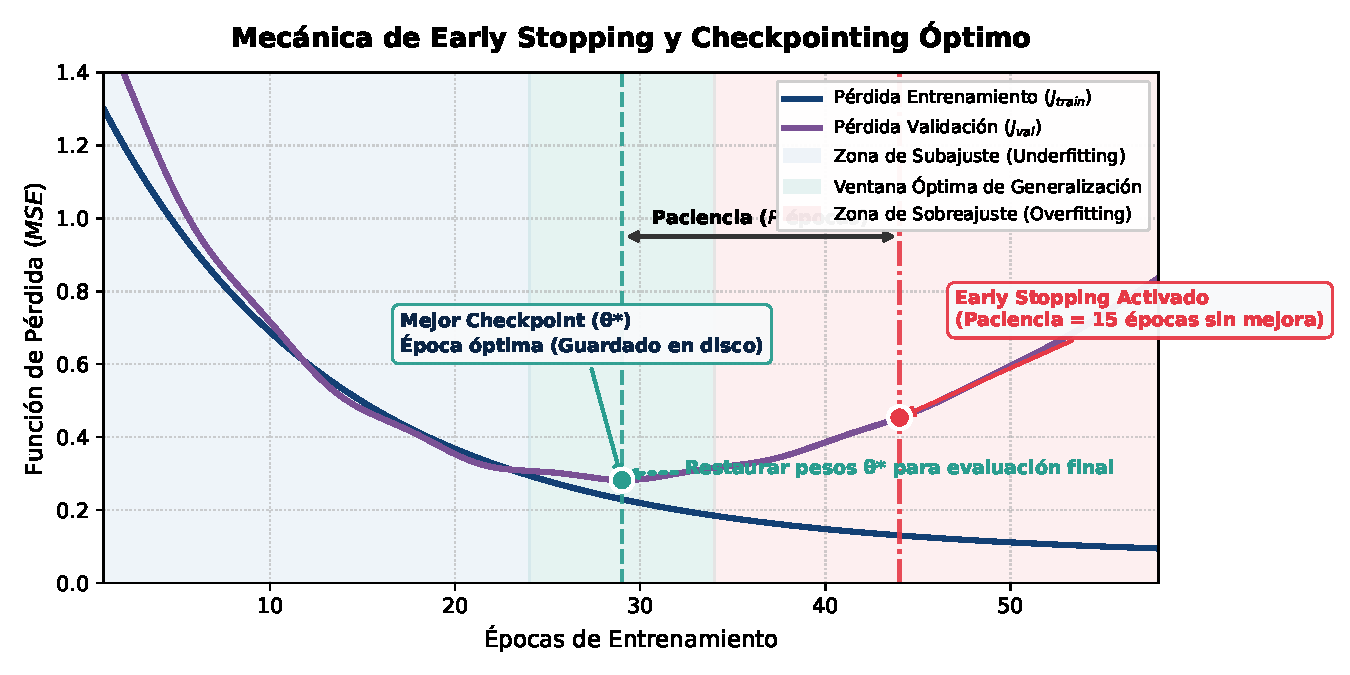
\includegraphics[width=0.76\textwidth,height=0.45\textheight,keepaspectratio]{esquema_early_stopping.pdf}
  \end{center}
  \vspace{-0.25cm}
  \begin{columns}[T]
    \begin{column}{0.32\textwidth}
      \textbf{1. Checkpoint Óptimo ($\theta^*$)}
      \begin{itemize}\scriptsize
        \item Se guarda en disco en la época de menor $J_{\text{val}}$.
        \item Garantiza la máxima generalización empírica.
      \end{itemize}
    \end{column}
    \begin{column}{0.34\textwidth}
      \textbf{2. Ventana de Paciencia ($P$)}
      \begin{itemize}\scriptsize
        \item Margen de tolerancia (ej. $15$ épocas).
        \item Evita detenerse ante ruido térmico del mini-batch.
      \end{itemize}
    \end{column}
    \begin{column}{0.32\textwidth}
      \textbf{3. Restauración de Pesos}
      \begin{itemize}\scriptsize
        \item Tras la parada, se descarta $\theta_{\text{stop}}$.
        \item Se carga $\theta^*$ para evaluar en datos de prueba.
      \end{itemize}
    \end{column}
  \end{columns}
\end{frame}

% -----------------------------------------------------------------------------
% SLIDE 5: IMPLEMENTACIÓN EN PYTORCH (CÓDIGO CLAVE)
% -----------------------------------------------------------------------------
\begin{frame}{Implementación en \texttt{red\_neuronal.py}}
  \begin{columns}[T]
    \begin{column}{0.48\textwidth}
      \begin{block}{1. Monitoreo y Guardado de Checkpoint}
        \scriptsize
\textbf{En cada época $t$:}
\begin{enumerate}
  \item Calcular $J_{\text{val}}$ sin gradientes (\texttt{torch.no\_grad()}).
  \item Si $J_{\text{val}} < J_{\text{val}}^{\min} - \delta$:
  \begin{itemize}\scriptsize
    \item $J_{\text{val}}^{\min} \leftarrow J_{\text{val}}$
    \item $t^* \leftarrow t$
    \item \texttt{torch.save(red.state\_dict(), "mejor\_modelo.pth")}
    \item Reiniciar contador: \texttt{epocas\_sin\_mejora = 0}
  \end{itemize}
  \item En caso contrario:
  \begin{itemize}\scriptsize
    \item \texttt{epocas\_sin\_mejora += 1}
  \end{itemize}
\end{enumerate}
      \end{block}
    \end{column}

    \begin{column}{0.48\textwidth}
      \begin{block}{2. Condición de Parada y Carga Óptima}
        \scriptsize
\textbf{Condición de parada anticipada:}
\begin{itemize}
  \item Si \texttt{epocas\_sin\_mejora >= PACIENCIA}:
  \begin{itemize}\scriptsize
    \item Imprimir diagnóstico de detención.
    \item Ejecutar \texttt{break} para salir del bucle.
  \end{itemize}
\end{itemize}

\vspace{0.1cm}
\textbf{Carga del mejor checkpoint antes del test:}
\begin{itemize}
  \item \texttt{red.load\_state\_dict(torch.load("mejor\_modelo.pth"))}
  \item \texttt{red.eval()}
  \item Predicción sobre \texttt{X\_prueba\_tensor}.
\end{itemize}
      \end{block}
    \end{column}
  \end{columns}
\end{frame}

% -----------------------------------------------------------------------------
% SLIDE 6: RESULTADO EN NUESTRA CURVA DE APRENDIZAJE
% -----------------------------------------------------------------------------
\begin{frame}{Curva de Aprendizaje Real con Early Stopping}
  \begin{columns}[c]
    \begin{column}{0.44\textwidth}
      \begin{center}
        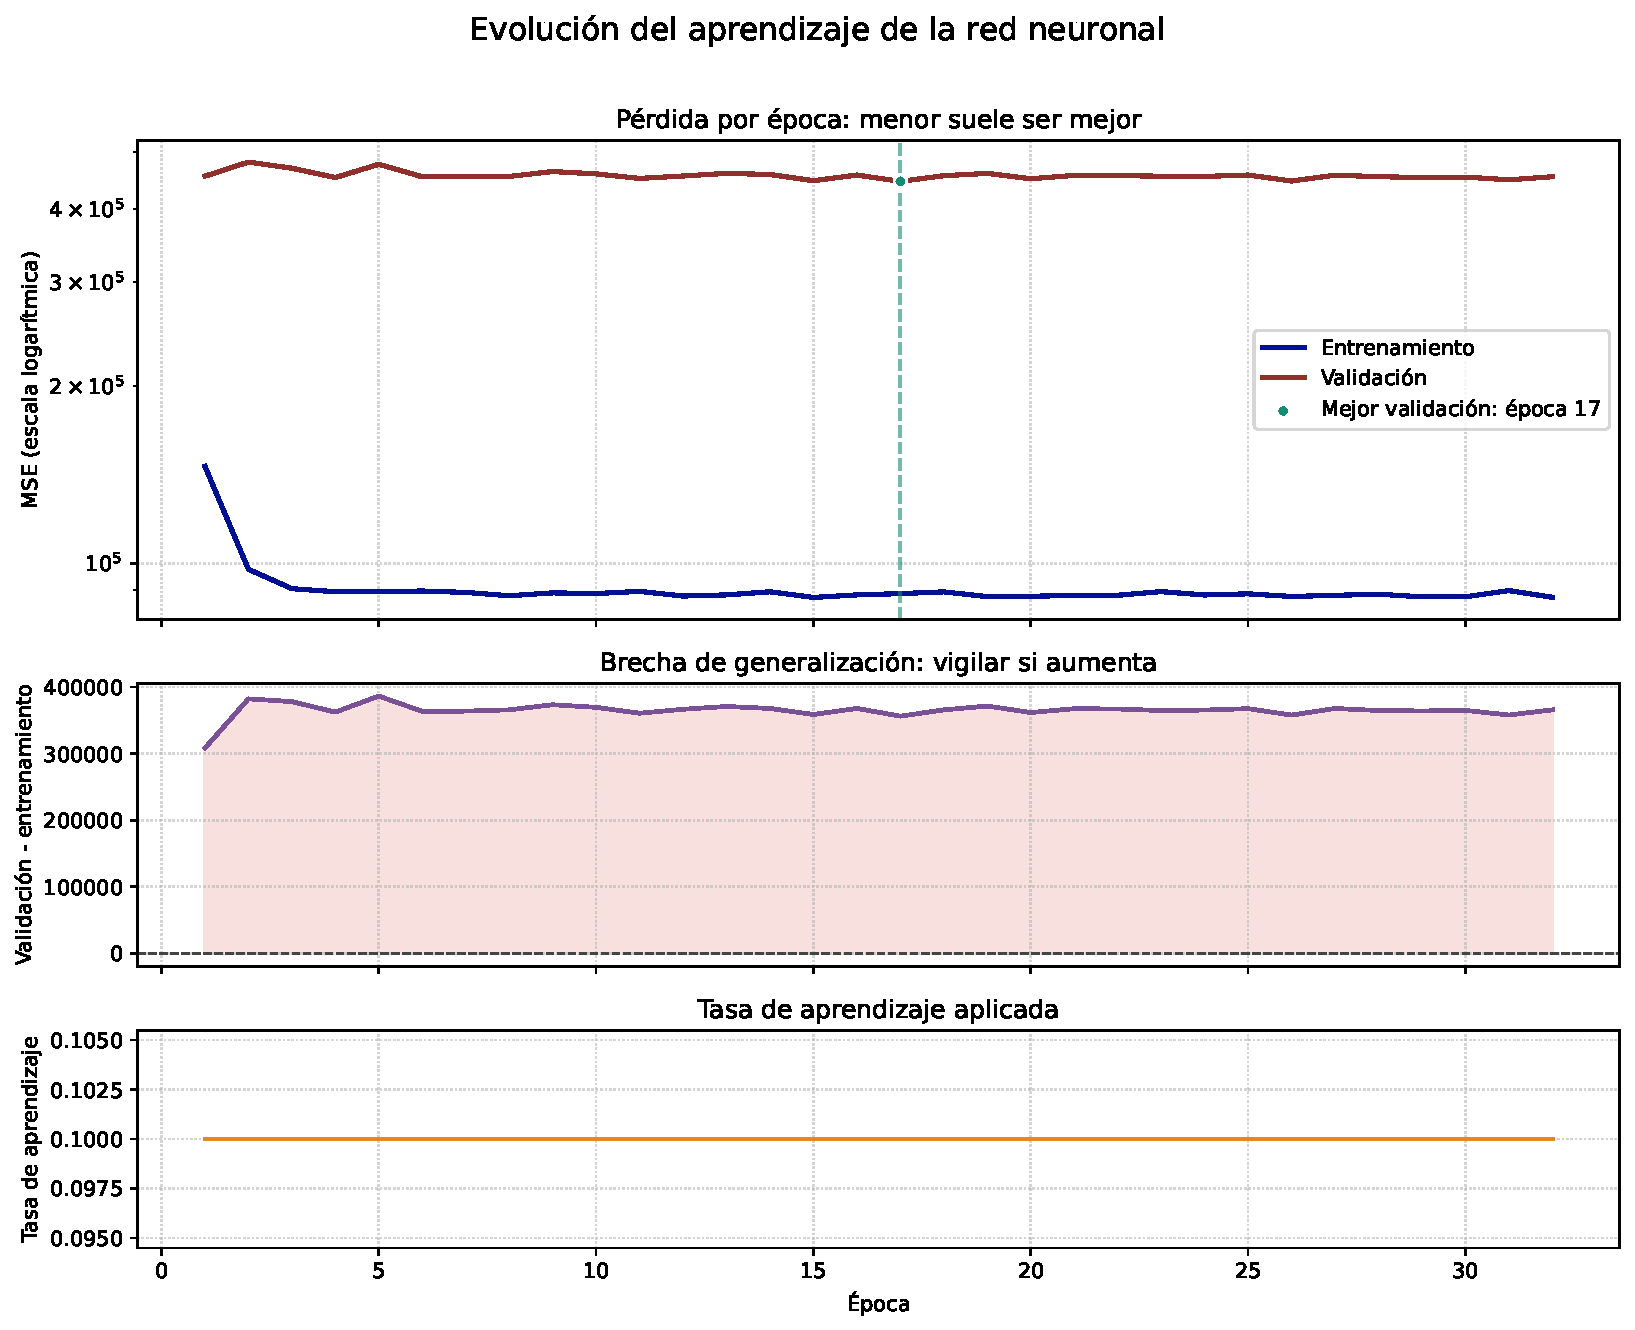
\includegraphics[height=0.78\textheight,keepaspectratio]{curva_aprendizaje.pdf}
      \end{center}
    \end{column}

    \begin{column}{0.54\textwidth}
      \begin{block}{Observación Experimental}
        \scriptsize
        \begin{itemize}
          \item \textbf{Mejor Época Registrada}: \textbf{Época 17} ($MSE_{\text{val}} = 445,235$).
          \item \textbf{Activación de Parada}: \textbf{Época 32} tras $15$ épocas consecutivas sin mejora ($\text{paciencia} = 15$).
          \item \textbf{Eficiencia y Ahorro}: Se evitaron $68$ épocas redundantes de cómputo.
        \end{itemize}
      \end{block}

      \vspace{-0.1cm}
      \begin{alertblock}{Diagnóstico de la Brecha ($\Delta J$)}
        \scriptsize
        \begin{itemize}
          \item En el panel central, la brecha de generalización ($\text{Val} - \text{Train}$) se estabilizó alrededor de la época 17.
          \item Continuar el descenso no reducía la cota superior del error de validación, confirmando que la red alcanzó su capacidad predictiva útil.
        \end{itemize}
      \end{alertblock}
    \end{column}
  \end{columns}
\end{frame}

% -----------------------------------------------------------------------------
% SLIDE 7: DIAGNÓSTICO VISUAL 1 — PREDICCIONES VS REALES
% -----------------------------------------------------------------------------
\begin{frame}{Diagnóstico Visual 1: Predicciones vs. Valores Reales}
  \begin{columns}[c]
    \begin{column}{0.56\textwidth}
      \begin{center}
        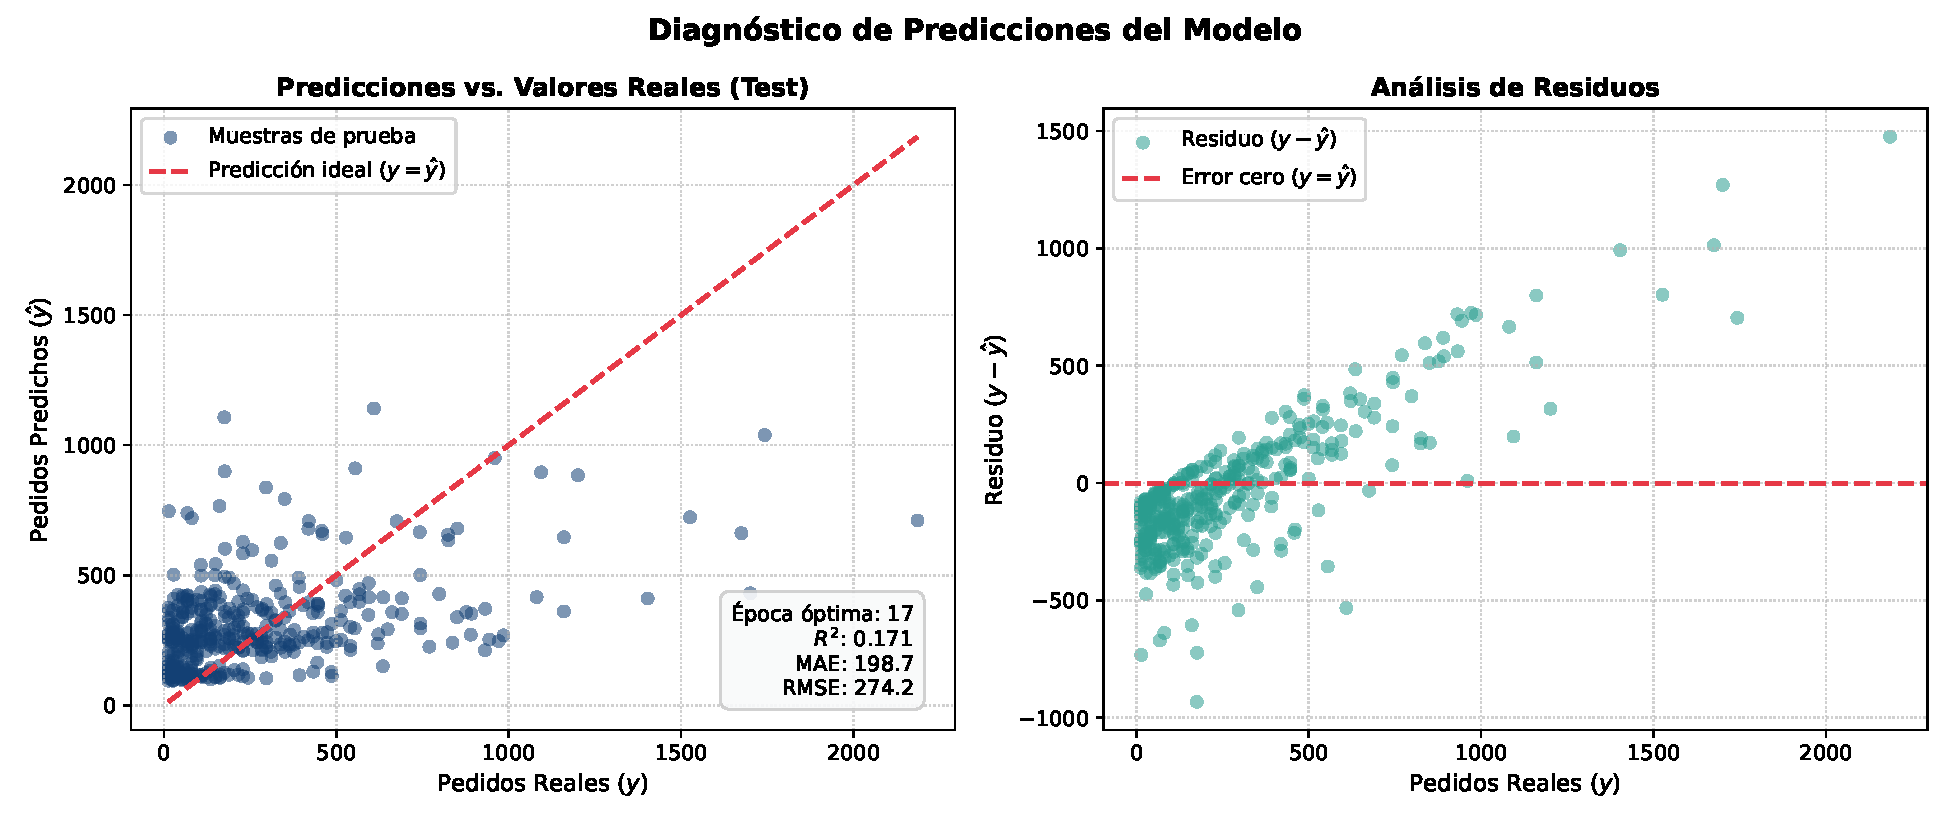
\includegraphics[width=\linewidth]{predicciones_vs_reales.pdf}
      \end{center}
    \end{column}

    \begin{column}{0.42\textwidth}
      \textbf{¿Qué nos revela esta gráfica?}
      \begin{itemize}\scriptsize
        \item \textbf{Línea de 45° ($y = \hat{y}$)}:
        Representa la predicción perfecta. Si el modelo fuera exacto, todos los puntos descansarían sobre la recta discontinua roja.
        \item \textbf{Dispersión en zona habitual ($< 1,000$ pedidos)}:
        La red captura la tendencia central con error acotado ($MAE \approx 198$).
        \item \textbf{Saturación en demandas extremas ($> 1,500$)}:
        Los pedidos inusualmente altos sufren subestimación. La red predice conservadoramente alrededor de $500$--$1,000$.
      \end{itemize}
    \end{column}
  \end{columns}
\end{frame}

% -----------------------------------------------------------------------------
% SLIDE 8: DIAGNÓSTICO VISUAL 2 — ANÁLISIS DE RESIDUOS
% -----------------------------------------------------------------------------
\begin{frame}{Diagnóstico Visual 2: Análisis de Residuos ($e_i = y_i - \hat{y}_i$)}
  \begin{center}
    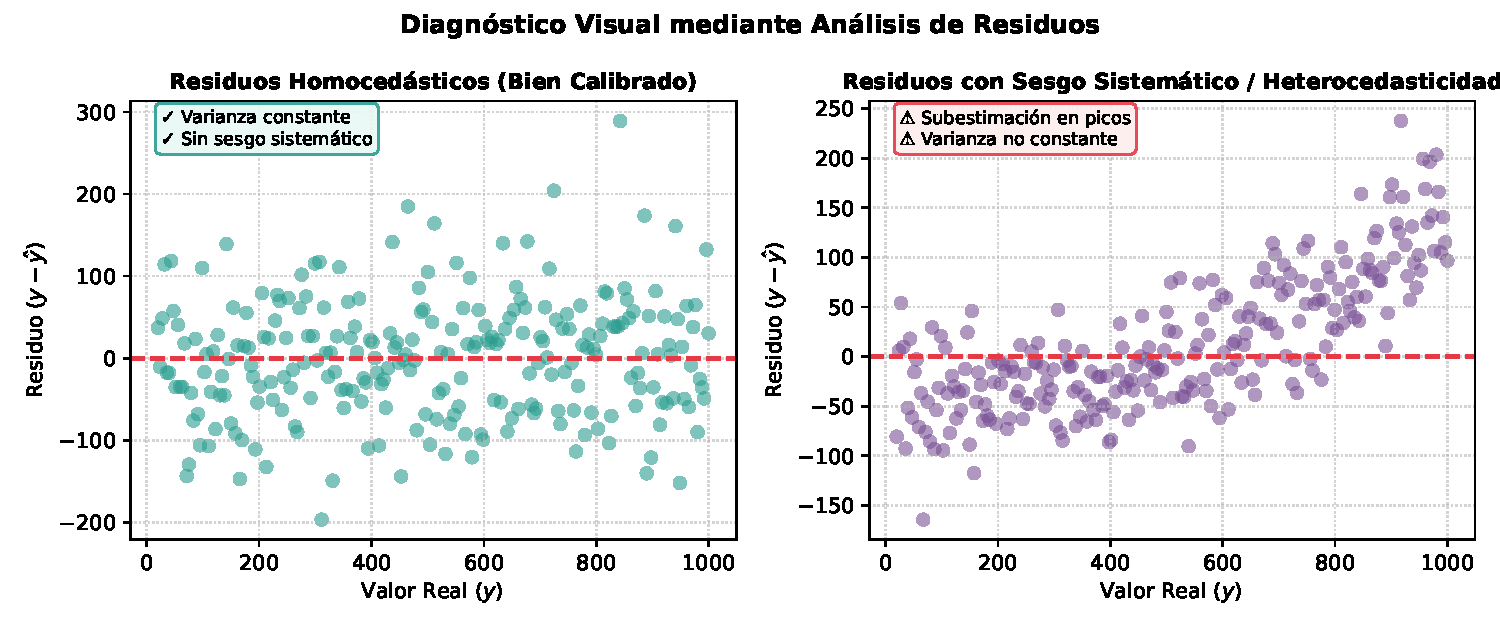
\includegraphics[width=0.76\textwidth,height=0.45\textheight,keepaspectratio]{analisis_residuos_teorico.pdf}
  \end{center}
  \vspace{-0.3cm}
  \begin{columns}[T]
    \begin{column}{0.48\textwidth}
      \textbf{Comportamiento Ideal (Homocedasticidad)}
      \begin{itemize}\scriptsize
        \item Los residuos forman una banda simétrica centrada en $0$.
        \item La varianza del error es constante independientemente de la magnitud de $y$.
        \item Garantiza que no hay información sistemática desperdiciada.
      \end{itemize}
    \end{column}
    \begin{column}{0.48\textwidth}
      \textbf{Comportamiento en Demanda Real (Heterocedasticidad)}
      \begin{itemize}\scriptsize
        \item En datasets de comida rápida, los picos masivos generan residuos positivos gigantes ($y \gg \hat{y}$).
        \item \textbf{Pauta de mejora}: Aplicar transformación logarítmica a la salida ($\log(1 + y)$) o función de pérdida Huber/Smooth L1.
      \end{itemize}
    \end{column}
  \end{columns}
\end{frame}

% -----------------------------------------------------------------------------
% SLIDE 9: LAS MÉTRICAS DE REGRESIÓN EXPLICADAS
% -----------------------------------------------------------------------------
\begin{frame}{Métricas de Desempeño: ¿Cómo se complementan?}
  \begin{center}
    \scriptsize
    \begin{tabular}{p{2.8cm} p{3.2cm} p{3.2cm} p{3.5cm}}
      \toprule
      \textbf{Métrica} & \textbf{Fórmula} & \textbf{Sensibilidad} & \textbf{Interpretación Práctica} \\
      \midrule
      \textbf{MAE} (Error Absoluto) &
      $\frac{1}{N}\sum |y_i - \hat{y}_i|$ &
      Lineal; robusto a valores atípicos &
      Magnitud intuitiva: \textit{«En promedio nos equivocamos en $\pm 198$ pedidos»}. \\
      \addlinespace
      \textbf{RMSE} (Raíz de MSE) &
      $\sqrt{\frac{1}{N}\sum (y_i - \hat{y}_i)^2}$ &
      Cuadrática; penaliza severamente errores grandes &
      Castiga desvíos en días pico: útil para gestión logística y rotura de stock. \\
      \addlinespace
      \textbf{Coeficiente $R^2$} &
      $1 - \frac{\sum (y_i - \hat{y}_i)^2}{\sum (y_i - \bar{y})^2}$ &
      Normalizado respecto a la varianza total &
      Porcentaje de variabilidad explicado ($1.0 = \text{perfecto}$, $0 = \text{promedio}$). \\
      \bottomrule
    \end{tabular}
  \end{center}

  \vspace{0.2cm}
  \begin{alertblock}{Lección del Diagnóstico}
    \scriptsize
    Un $R^2$ modesto en datos brutos ocurre por la enorme asimetría en pedidos extremos ($13$ a $12,137$).
    El análisis visual de residuos explica de inmediato lo que un único número tabular no puede revelar.
  \end{alertblock}
\end{frame}

% -----------------------------------------------------------------------------
% SLIDE 10: EL PIPELINE COMPLETO Y REGLAS DE CO-DISEÑO
% -----------------------------------------------------------------------------
\begin{frame}{Protocolo de Ingeniería en Aprendizaje Supervisado}
  \begin{center}
    \begin{tikzpicture}[
      scale=0.82, every node/.style={transform shape},
      fase/.style={rectangle, rounded corners, minimum width=2.5cm, minimum height=1.0cm, align=center, draw=NavyDark, fill=SandLight, font=\scriptsize\bfseries},
      flecha/.style={thick, ->, color=NavyMedium}
    ]
      \node (split) [fase, fill=NavyMedium!15] {1. Split 3 Vías\\Train / Val / Test};
      \node (scale) [fase, right=0.35cm of split] {2. Escalado\\Fit en Train};
      \node (train) [fase, right=0.35cm of scale, fill=TealAccent!20] {3. Bucle PyTorch\\Gradientes en Train};
      \node (early) [fase, right=0.35cm of train, fill=CoralAccent!20] {4. Early Stopping\\Guardar Checkpoint};
      \node (eval)  [fase, right=0.35cm of early, fill=NavyDark, text=white] {5. Inferencia Final\\Cargar $\theta^*$ y Eval};

      \draw [flecha] (split) -- (scale);
      \draw [flecha] (scale) -- (train);
      \draw [flecha] (train) -- (early);
      \draw [flecha] (early) -- (eval);
    \end{tikzpicture}
  \end{center}

  \vspace{0.2cm}
  \begin{columns}[T]
    \begin{column}{0.48\textwidth}
      \begin{block}{Buenas Prácticas de Paciencia}
        \scriptsize
        \begin{itemize}
          \item Si el batch size $B$ es pequeño (más ruido de gradiente), \textbf{aumentar la paciencia} ($P \ge 20$).
          \item Si usamos un optimizador adaptativo con decay (ej. scheduler), sincronizar la paciencia con la reducción de tasa.
        \end{itemize}
      \end{block}
    \end{column}

    \begin{column}{0.48\textwidth}
      \begin{block}{Integridad Metodológica}
        \scriptsize
        \begin{itemize}
          \item \textbf{Cero fuga de información}: El test set jamás interviene en la decisión de detenerse ni en el escalado.
          \item \textbf{Determinismo}: La semilla fija (\texttt{seed 42}) garantiza experimentos rigurosamente reproducibles.
        \end{itemize}
      \end{block}
    \end{column}
  \end{columns}
\end{frame}

% -----------------------------------------------------------------------------
% SLIDE 11: CONCLUSIONES
% -----------------------------------------------------------------------------
\begin{frame}{Conclusiones y Siguientes Pasos}
  \begin{columns}[T]
    \begin{column}{0.48\textwidth}
      \begin{block}{Lo que Hemos Consolidado}
        \scriptsize
        \begin{enumerate}
          \item \textbf{Control de sobreajuste}: Early stopping detiene el cómputo en el punto de óptima generalización empírica.
          \item \textbf{Checkpointing persistente}: El archivo \texttt{mejor\_modelo.pth} conserva el estado óptimo $\theta^*$ listo para despliegue.
          \item \textbf{Diagnóstico integral}: La doble gráfica (predicciones vs reales y análisis de residuos) permite entender dónde y por qué falla el modelo.
        \end{enumerate}
      \end{block}
    \end{column}

    \begin{column}{0.48\textwidth}
      \begin{alertblock}{La Continuación Natural Próxima}
        \scriptsize
        \begin{itemize}
          \item \textbf{Transformación de la variable objetivo}: Aplicar $\log(1 + y)$ para comprimir la varianza extrema de los pedidos.
          \item \textbf{Regularización adicional}: Probar \texttt{Dropout(0.2)} o penalización $L_2$ (\texttt{weight\_decay}).
          \item \textbf{Módulo de Inferencia en Producción}: Crear una función \texttt{predecir\_pedido(precio, promo, semana)} para responder consultas operativas.
        \end{itemize}
      \end{alertblock}
    \end{column}
  \end{columns}
\end{frame}

% -----------------------------------------------------------------------------
% SLIDE 12: CIERRE
% -----------------------------------------------------------------------------
\begin{frame}[standout]
  \Huge ¿Preguntas o Discusión?
  \vspace{0.4cm}

  \normalsize Código fuente: \texttt{red\_neuronal.py} y \texttt{graficar\_aprendizaje.py} \\
  Pesos óptimos guardados: \texttt{mejor\_modelo.pth}
\end{frame}

\end{document}
